\documentclass[compsoc]{IEEEtran}
\usepackage{graphicx}
\usepackage{amsmath}
\usepackage{authblk}
\usepackage[english]{babel}
\usepackage{blindtext}

\usepackage[ruled,vlined,linesnumbered]{algorithm2e}
\usepackage{algorithmic,float}
\usepackage{setspace}
\usepackage{amsfonts}
%\usepackage{hyperref}
\graphicspath{ {./images/} }
\usepackage{subfig}
\usepackage{fontspec}
\usepackage{listings}
\usepackage{amsmath}
\usepackage{mathabx}
\usepackage[bottom]{footmisc}
\newfontfamily\listingsfont[Scale=.7]{inconsolata}\usepackage[font=footnotesize,labelfont=bf]{caption}
\captionsetup[algorithm2e]{font=footnotesize}
\usepackage[table,xcdraw]{xcolor}
\usepackage[utf8]{inputenc}
\title{Assignment: Regularization techniques and Autoencoder on Multi-MNIST dataset}
\author{David Bertoldi -- 735213 \\ email: d.bertoldi@campus.unimib.it}
\affil{Department of Informatics, Systems and Communication}
\affil{University of Milano-Bicocca}
\date{October 2022}


\begin{document}

\maketitle 

\section{Inspecting the data}
The data provided consinst of a set of grey-scale images containing 2-digits handwrittend numbers.
The source is a modification of the MNIST dataset: each image is composed by two digits coming from
the original MNIST that may be overlapped in different intensity. This let expand the dataset from
the set of numbers from 0 to 9 to numbers from 1 to 50. \par

Figure \ref{fig:sample} shows the first 16 samples of the training dataset with unique labels.

\begin{figure}[ht!]
\centering                                                                        
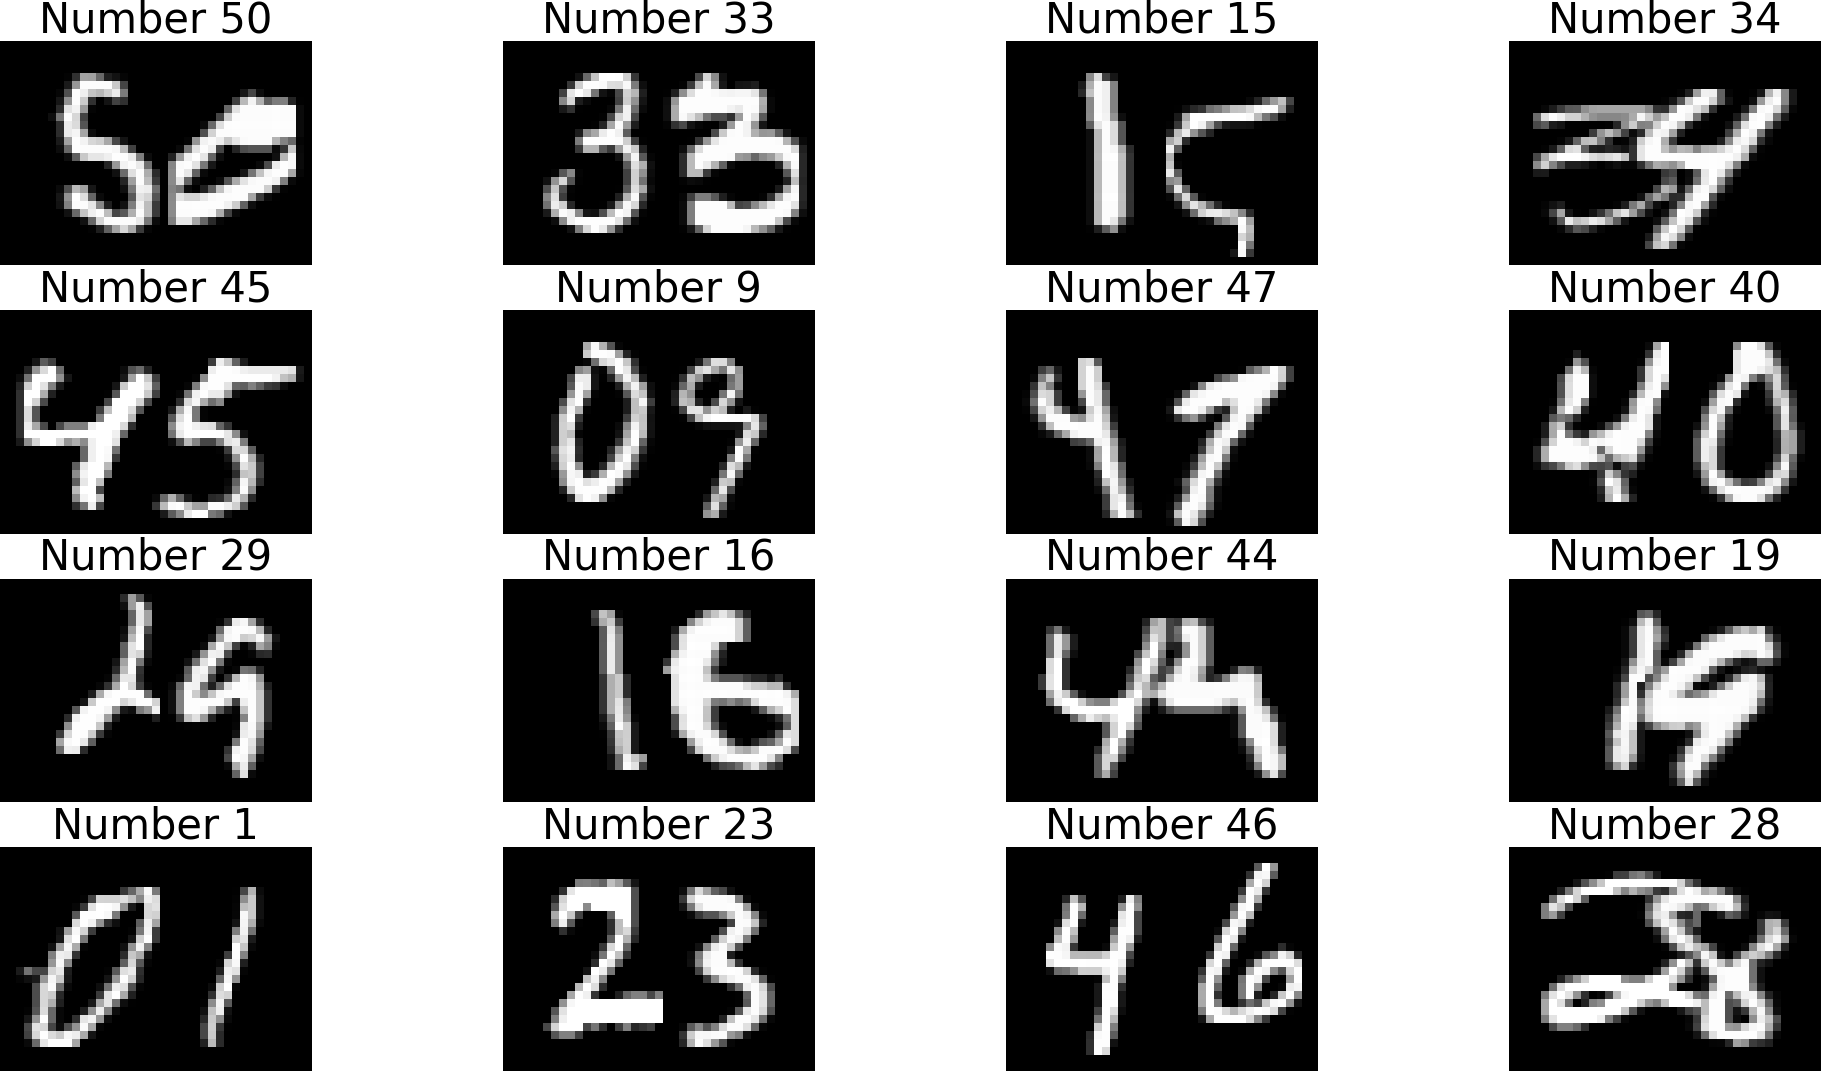
\includegraphics[width=3.5in]{sample.png}
\captionsetup{justification=centering}                                                                                                                                   
\caption{Sample of the first 16 unique samples}
\label{fig:sample}
\end{figure}

The data is already divided in training and test datasets. The first present a non-uniform distribution,
as shown in Figure \ref{fig:datahist}. 
Many numbers have very low occurrencies, like 43 with 117 or 17 with 130, against other like 11 with 3112 or 19 with 2890.
As a matter o fact the train dataset has mean $\mu\simeq 1671$ with a standard deviation $\sigma\simeq 1045$, leading to
an unbalanced training for some classes.

\begin{figure}[ht!]
\centering                                                                        
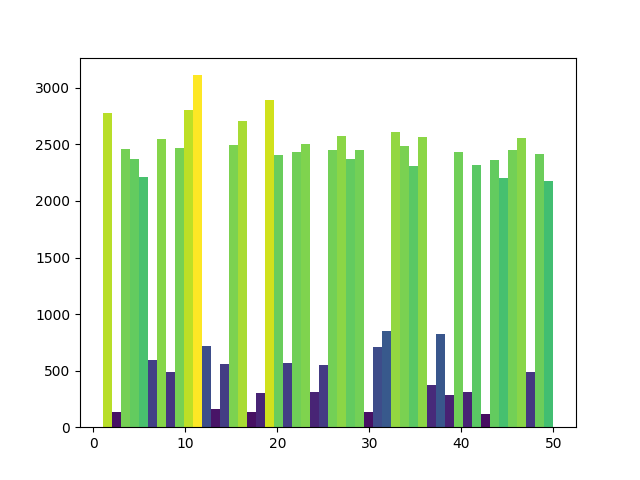
\includegraphics[width=3.5in]{datahist.png}
\captionsetup{justification=centering}                                                                                                                                   
\caption{Histogram of the frequency of samples in the dataset}
\label{fig:datahist}
\end{figure}


Along with the bias of the dataset, some number at first sight are difficult to interpret even for the human mind. For example,
Figure \ref{fig:unread} shows 6 difficult numbers to read. \par

Before training a FFNN using this images, encoded in $28\times39$ matrices with values from $0$ to $255$, we flattened them in
arrays $1\times1092$ and rescaled each value in the continuous interval $[0, 1]$.

\begin{figure}[ht!]
\centering                                                                        
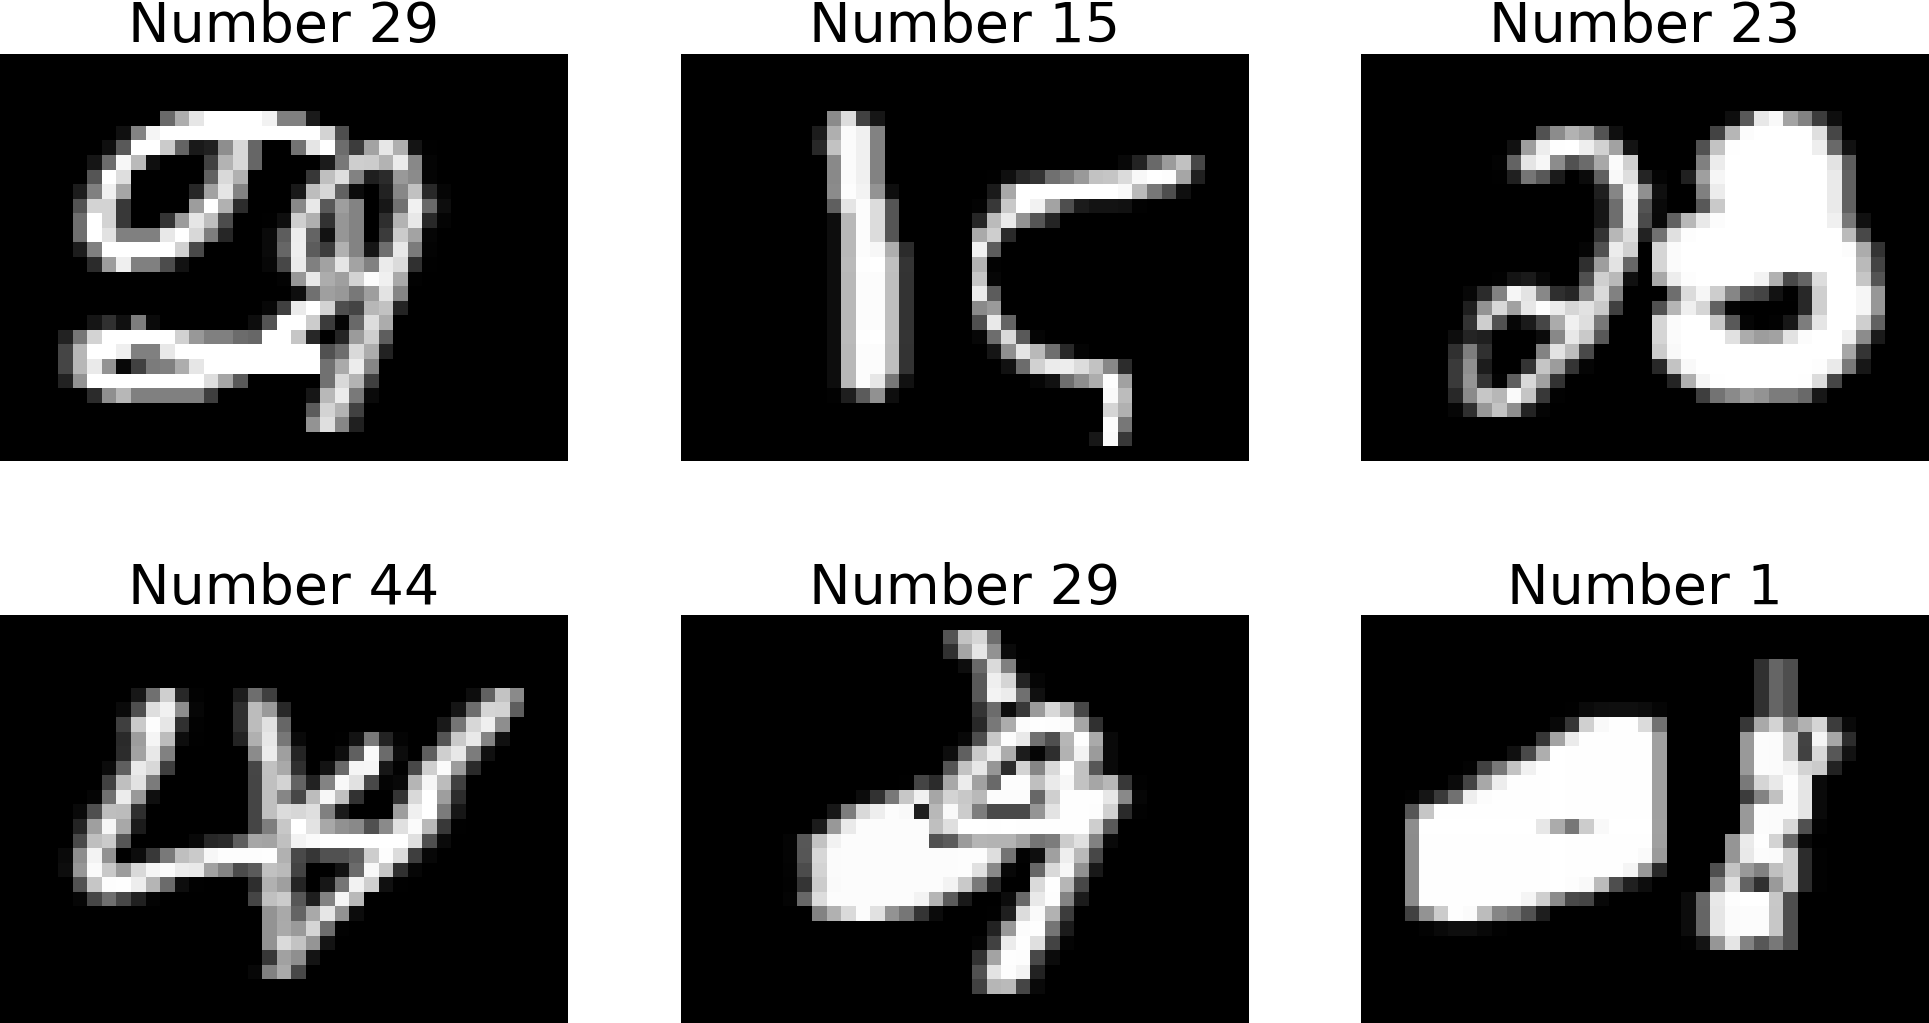
\includegraphics[width=2.5in]{unread.png}
\captionsetup{justification=centering}                                                                                                                                   
\caption{Difficult to read numbers}
\label{fig:unread}
\end{figure}


\section{Preparing the data}
As said in the section before, the dataset is divided into training and test samples. A validation subset is missing and thus
is retrieved from the training set: $20\%$ of the images are randomly used for validation instead of training (along with their labels). \par
About labels, we encoded them in one-hot vectors so that the $1$ are set in the index representing the numerical class.

Another, technical, issue is that \texttt{np\_utils.to\_categorical}, used to create the one-hot vectors, generates 51 classes instead of 50. That's because the function creates as many classes as the highest value inside the input plus one: it takes for granted that we were using a zero-based index. In order
to overcome this, without writing that function from scratch, we subracted 1 to each element of each vector inside the training and test label set.
Obvisously that operation is reverted when trying to predict the values.


\section{Unregularized FFNN}

The aim of this section is to describe a FFNN with less than $100.000$ parameters that is able to classify
with high level of accuracy the numbers from the dataset without any regularization technique. 

\subsection{The network}
Because the number of parameters
are partially determined by the size of the input and output, we tested a FFNN with 2, 3, 4 and 5 hidden layers, but we found that 2-layers model
generalized better over a deeper (and less wide) model. Without entering in the details, the deepest model had 5 layers with 70 to 50 neurons each.\par 


We found a good spot with 80 neurons in the first layer and 50 in the seconds, for a total of 96.660 parameters. 
Figure \ref{fig:noregffnn} shows the architecture of the network used in this section.






\begin{figure}[ht!]
\centering                                                                        
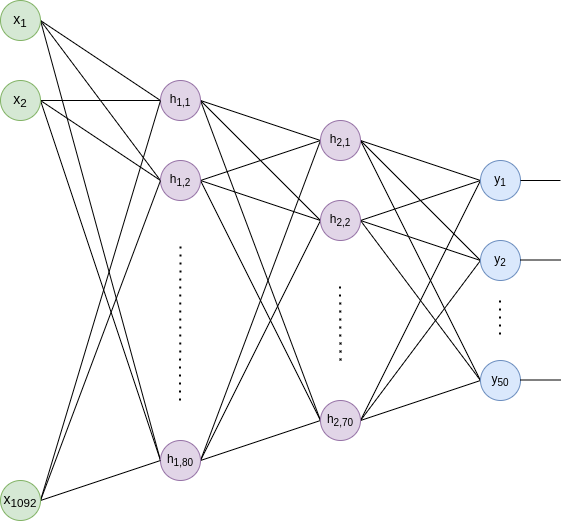
\includegraphics[width=2.5in]{noregffnn.png}
\captionsetup{justification=centering}                                                                                                                                   
\caption{Architecture of the unregularized network}
\label{fig:noregffnn}
\end{figure}

Each hidden neuron uses \texttt{Sigmoid} as activation function. We tried \texttt{LeakyReLU} with $\alpha=0.01$ as well but resulting in a divergence in the model (the validation loss kept tp slighty grow after 15 epochs). The source was probably the explosion of the gradient caused by the function.  \par 
The output layer computes a \texttt{Softmax}, which converts an input vector of real values to an output vector that can be interpreted as categorical probabilities.

\subsection{Training}
The choice of the optimizer was among \emph{SGD}, \emph{RMSProp} and
\emph{Adam}. This selection was influenced also by the initialization of the weights: 
\emph{SGD} performed well with \texttt{GlorotNormal} (Xavier) initializer but not as well as \emph{RMSProp} and
\emph{Adam} with \texttt{HeNormal}. \emph{SGD} with \texttt{HeNormal} resulted in a model that couldn't converge at all.

We tried all of them and chose Adam with learning
rate of $10^{-3}$ , $\beta_1 = 0.9$ and $\beta_2 = 0.999$ because it seemed to
escape better from local minima, converging faster and giving
better accuracy. \par 
Because we are trying to find which images best suits in one of the 50 classes, the best loss function is the \emph{Categorical Cross-Entropy}.\par
The batch size of 256 gave the best results: 512 was another good choice but the convergence was slower and lower values performed worse; that might be
due to the fact that the model needed a good amount of variety of information before every update. But even using mini-batches of 8 the validation accuracy
reached $89\%$.




\begin{figure}[ht!]
\centering                                                                        
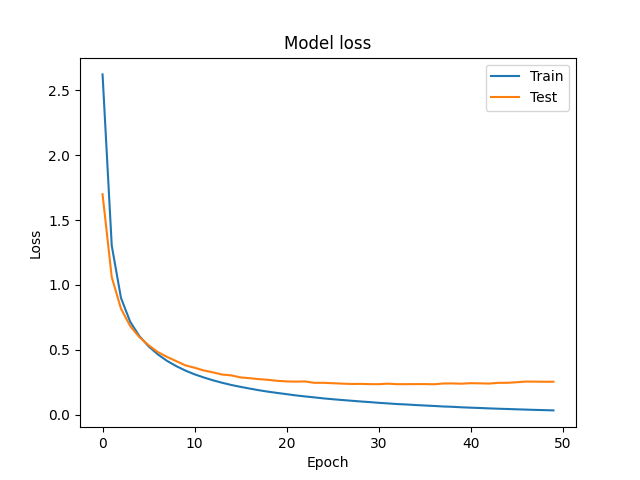
\includegraphics[width=3.5in]{../images/noreg/loss-sigmoid-categorical_crossentropy-Adam-50-256.png}
\captionsetup{justification=centering}                                                                                                                                   
\caption{Loss (unregularized)}
\label{fig:loss1}                                                                                                                                                           
\end{figure}


\begin{figure}[ht!]
\centering                                                                        
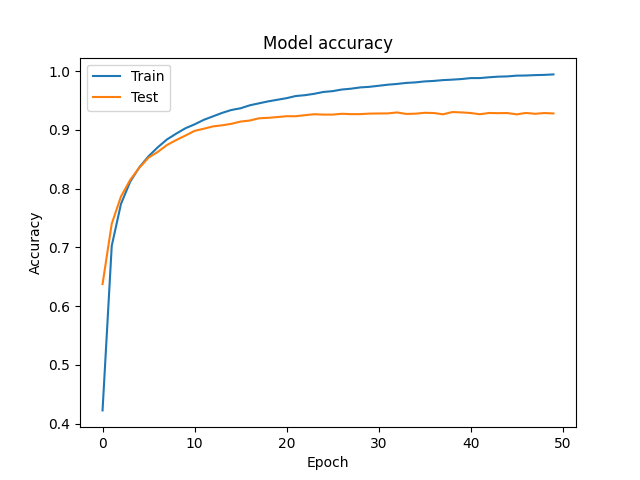
\includegraphics[width=3.5in]{../images/noreg/accuracy-sigmoid-categorical_crossentropy-Adam-50-256.png}
\captionsetup{justification=centering}                                                                                                                                   
\caption{Categorical accuracy (unregularized)}
\label{fig:acc1}                                                                                                                                          
\end{figure} 

We choose 50 as number of epochs in order to see the effects of missing regularization like \emph{early stopping}, 
even if the model reached an optimal state after 10 epochs.
As shown in Figure \ref{fig:loss1} and \ref{fig:acc1} it is possible to see that the training validation reached $\sim100\%$ which means the model
overfitted so much that almost memorized the training set. 
As metric we used the \emph{categorical accuracy} because calculates the percentage of predicted values that match with true values for one-hot labels.


\subsection{Evaluation}
\begin{figure}[ht!]
\centering                                                                        
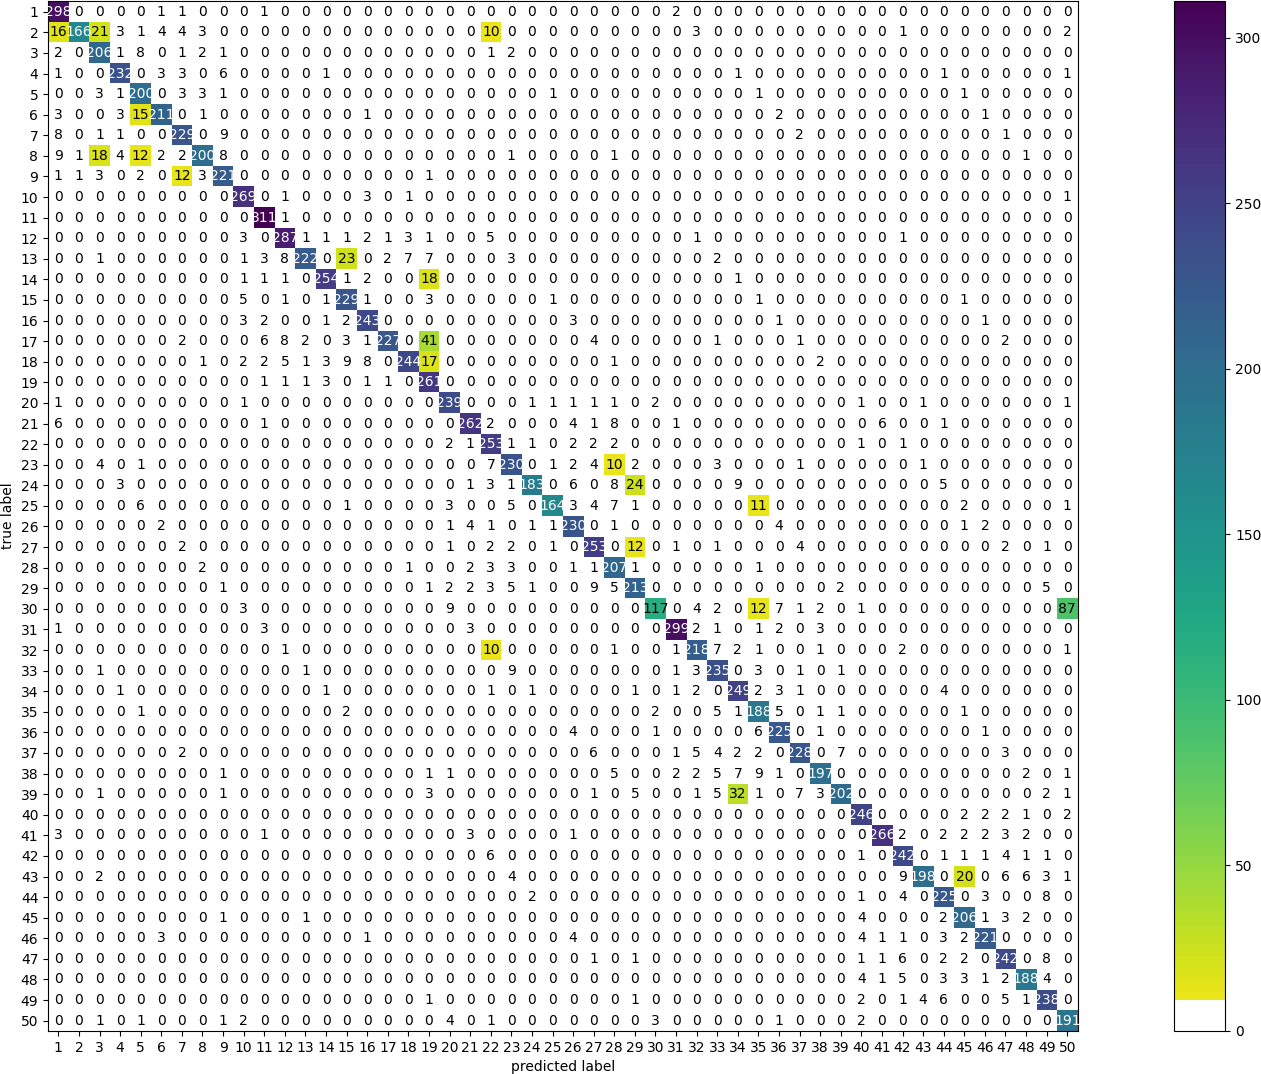
\includegraphics[width=3.5in]{noregcm.png}
\captionsetup{justification=centering}                                                                                                                                   
\caption{Confusion matrix of the evaluation of the test set (unregularized network)}
\label{fig:noregcm}                                                                                                                                                           
\end{figure}
The validation accuracy reached $91,5\%$ after 14 epochs and remained stable till the end. The categorical accuracy 
over the test set reached $89\%$ and can be analyzed with the help of the confusion matrix (Figure \ref{fig:noregcm}). 
The confusion matrix uses a custom colormap (a \emph{viridis} but with the first 10 values set to 0) so that was easier
to hide negligible errors (in this case, less than 10 mismatches). It is noticeable that the model confuses number 50 with 30,
19 with 17, 34 with 39 and others. These errors are not only due to the similarity between their digits, but because
these are the classes with less elements in the training set. So with no surprise the unbalances inside the training set played an
important role.

\par





\section{Regularized FFNN}
The aim of this section is to describe a FFNN with less than $100.000$ parameters that is able to classify
with high level of accuracy the numbers from the dataset with one or more regularization technique. 

\subsection{The network}
In order to better measure the effects of regularization we used the very same architecture as base (2 layers, 80 and 70 neurons).


\subsection{Regularization techniques}
In this section we describe the techiques tested, used or discarded to achieve a lower level of underfitting and secondary to reach a better level of accuracy.

\subsubsection{Data augmentation}
The first attempt of undirect regularization involved filling the gap between the classes by generating new samples for the less populated classes. The procedure, described in Algorithm \ref{alg:aug}, generates for each class as many samples as there are in the percentage $p$ of the difference with the most populated class.
By choosing $p=10\%$ each class diminuishes the gap with the major class by $10\%$. \par
Three techniques were taken in account: \emph{adding noise}, \emph{image shifting} and \emph{image rotation}. The first added a gaussian noise $\mathcal{N}(0, \frac{1}{2})$, the second randomly shifted the image along the 2 axis by 2 in both directions and the third rotated the image by a random angle bewteen $-20^{\circ}$ and $20^{\circ}$. \par
None of the above helped the network: the level of accuracy dropped to $86\%$ and the loss was very high when applying noise ($\geq 0.6$). Image roation alone is the only one that didn't make the accuracy worse. For these reasons data augmentation was discarded even if theoretically speaking filling the gap between samples makes sense. Probably the model already recognized single features for those samples so that adding similar samples just increased redundancy.

\begin{algorithm}[h]
\SetAlgoLined
\KwData{\emph{$X$ training samples}, \emph{$Y$} training labels, $p \in \mathbb{N}$}
\KwResult{\emph{$X$}, \emph{$Y$} }
$l=|Y|$\;
$C \gets \{\}$\;
\For{$i \gets 0$ \textbf{to} $l$}{
\eIf{$Y_i \in C$}{
$C_i \gets C_i + 1$\;
}{
$C_i \gets 1$\;
}
}


$m \gets \max_k C_k$\;

\For{$(k,v) \in C$}{
$S = \{e \in X : e = k\}$\;
$g \gets \left \lfloor \frac{m - v}{p} \right \rfloor$\;
\For{$i \gets 0$ \textbf{to} $g$}{
$x \gets augment(S_{random})$\;
$\text{append } x \text{ to } X$\;
$\text{append } k \text{ to } Y$\;
}
}
\Return $shuffle(X, y)$\;

\caption{Data augmentation algorithm}\label{alg:aug}
\end{algorithm}


\subsubsection{L1 and L2}
\emph{L1} and \emph{L2} are typical techniques used to reduce the overfitting of the model by settings penalties in the coeffiecients. We tried first \emph{L1}, but even with low regularization factors (from $10^{-3}$ to $10^{-5}$) the model underfitted too much. \emph{L2} with a regularization factor of $10^{-5}$ performed better, similar to a a regularization factor of $10^{-4}$ and a learning rate 10 times higher ($10^{-2}$), but was outperformed in accuracy by a model non implementing it.

\subsubsection{Dropout}
Dropout turned out to be a good choice: it dropped the overfitting without losing too much accuracy. We chose a drop out probability for each layer of $10\%$ because the network wasn't too big and higher probabilities gave worse results. This strategy helped the network to ignore certain features of the images or the $0s$ of the matrices (black spaces). A representation of the network can be found in Figure \ref{fig:regffnn}. 

\begin{figure}[ht!]
\centering                                                                        
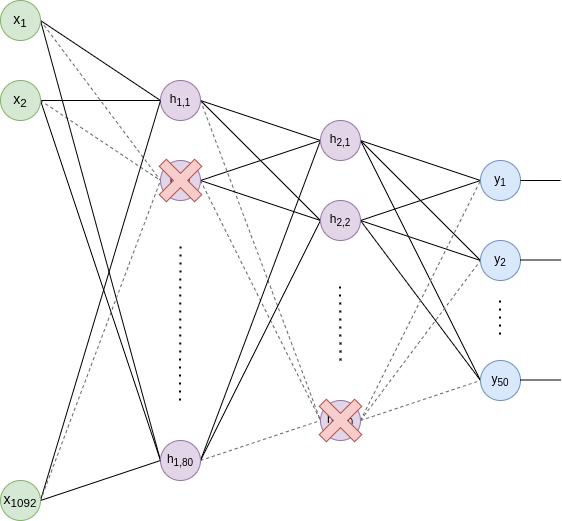
\includegraphics[width=2.5in]{regffnn.png}
\captionsetup{justification=centering}                                                                                                           
\caption{Architecture of the network with dropout}
\label{fig:regffnn}
\end{figure}

\subsubsection{Early stopping}
Another game changer was the application of \emph{early stopping} on the validation, with a patience of 10 epochs and $\delta = 0.05$. This greately reduced the overfitting and because the model converged after 15-20 epochs we restored the weights to the last best snapshot ($20^{\text{th}}$ epoch).




\subsection{Training}
The optimizer used was \emph{Adam} with a learning rate of $10^{-3}$ in conjuction with $\texttt{HeNormal}$ initializer. We used 50 epochs and batches of 256 elements 
not only to replicate the methodologies used with the unregularized model, but because outperformed other configurations. This means that the addition of dropout hasn't changed the quantity of information needed by the model before an update.



\begin{figure}[ht!]
\centering                                                                        
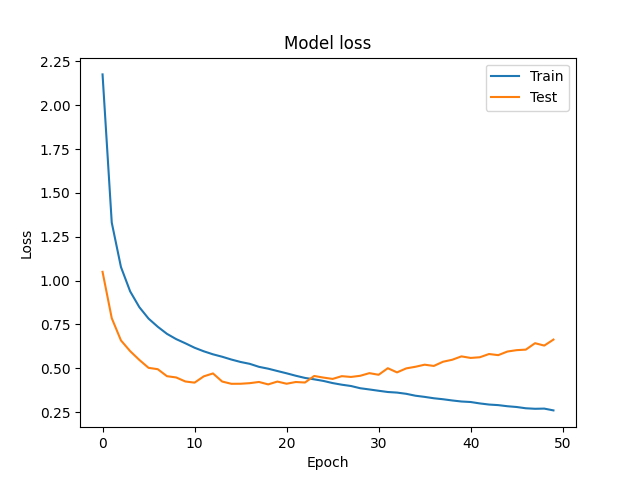
\includegraphics[width=3.5in]{../images/reg/loss-LeakyReLU-NoneType-categorical_crossentropy-Adam-50-256-0.1.png}
\captionsetup{justification=centering}                                                                                                                              
\caption{Loss (unregularized)}
\label{fig:loss2}                                                                                                                                         
\end{figure}


\begin{figure}[ht!]
\centering                                                                        
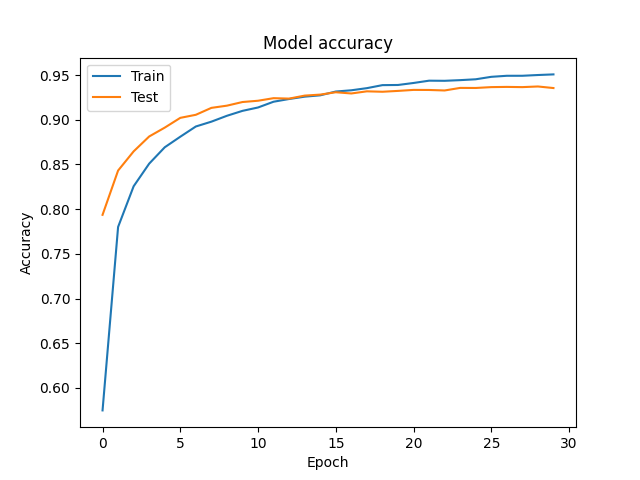
\includegraphics[width=3.5in]{../images/reg/accuracy-LeakyReLU-NoneType-categorical_crossentropy-Adam-50-256-0.1.png}
\captionsetup{justification=centering}                                                                                                                            
\caption{Categorical accuracy (unregularized)}
\label{fig:acc2}                                                                                                                                          
\end{figure} 


\subsection{Evaluation}

The validation accuracy reached $93\%$ ($+1.5\%$ over the unregularized model) but with a training accuracy of $94\%$: this means the model had not memorized the dataset
in favor of a better generalization. The test accuracy reached $92\%$ ($+3\%$) and this proved that the model implementing regularization techniques 
had a higher capabilities to generalize the problem. \par
The confusion matrix in Figure \ref{fig:regcm} shows the improvements made from the previous model: there are still some mismatches between predicted and true labels, but they have lower intensity \emph{i.e.} there are less cases where the $50$ is confused with $30$ ($-28\%$) or $19$ with $17$ ($-70\%$).\par
The regularization definetely changed the network performances without changing the architecture per se.

\begin{figure}[ht!]
\centering                                                                        
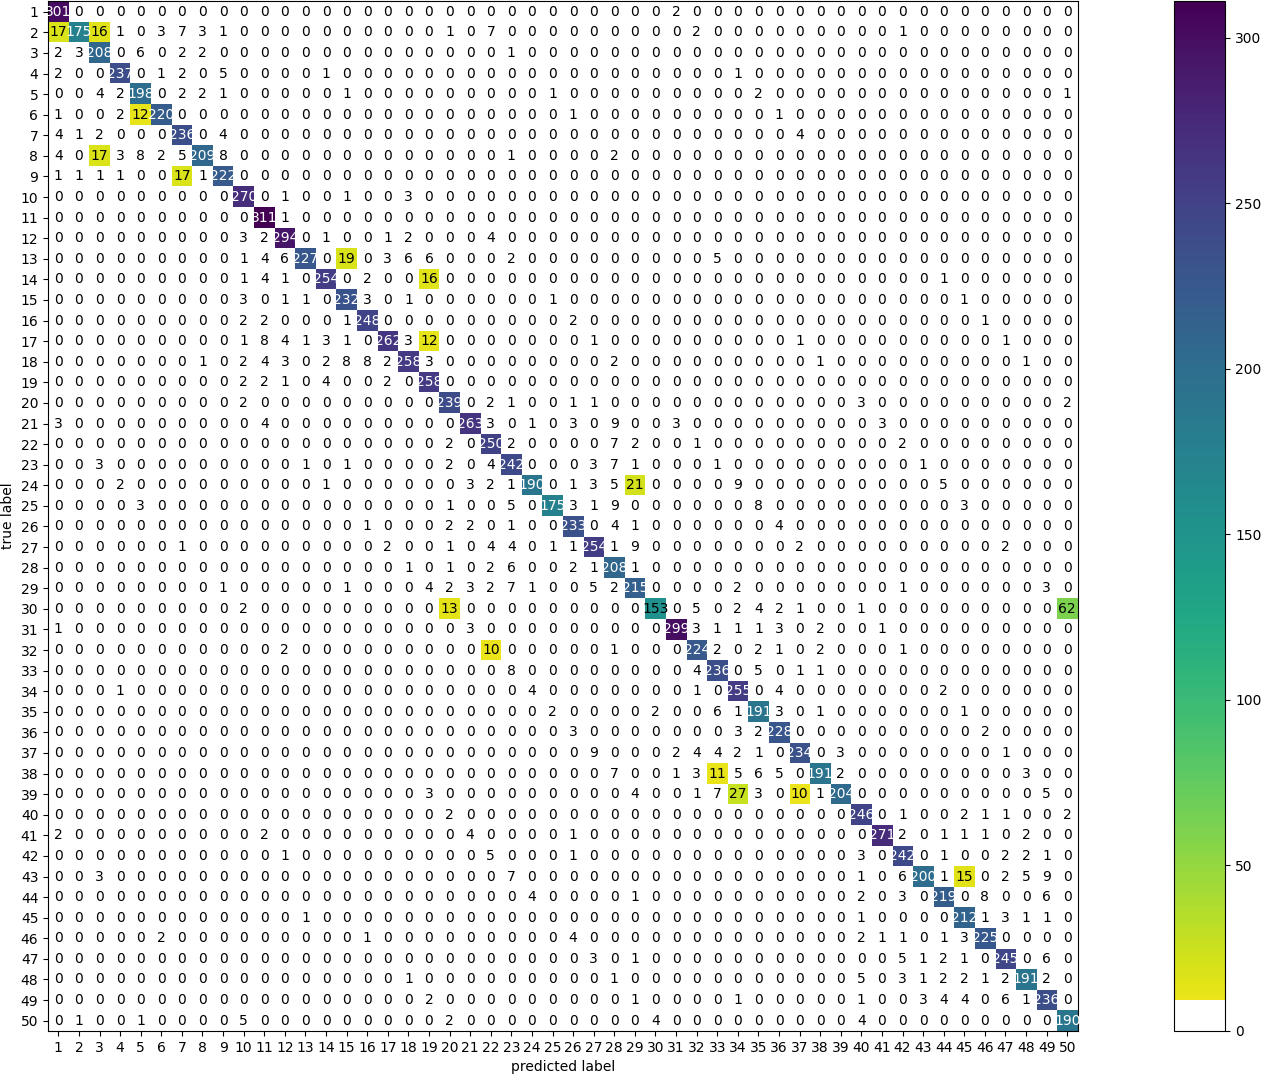
\includegraphics[width=3.5in]{regcm.png}
\captionsetup{justification=centering}
\caption{Confusion matrix of the evaluation of the test set (regularized network)}
\label{fig:regcm}
\end{figure}


\section{Autoencoding}
In this section we show how to build an autoencoder that compresses the knowledge of the original input and that reconstructs the input starting from the compessed (encoded) version.
\subsection{The nerwork}
Before deciding the compression rate, we describe here the foundamentals of the autoencoder's architecture. The input, like in the previous cases, is represented by a flatten version of the images, that is a $1\times1092$ array. Because it is an autoencoder, the same goes for the output. We chose 2 hidden layers for the encoding and 3 for decoding; we used this unbalancing since it easy for the network to compress information but harder to decompress them. So the decoding part uses a more complex model.\par
The compression factor that defines the lenght of the encoding had been decided with a benchmark: we trained 10 networks with different compression factors (from 20 to 30) and analyzed their mean squared errors. Figure \ref{fig:multiacc} and \ref{fig:mse} demonstrates that the best compression factor was 20, that is having an encoded layer formed by 54 layers. This was quite predictable but it is worth to notice how the MSE didn't linearly follow the compression rate; and this fact wasn't obvious.\par



\begin{figure}[ht!]
\centering                                                                        
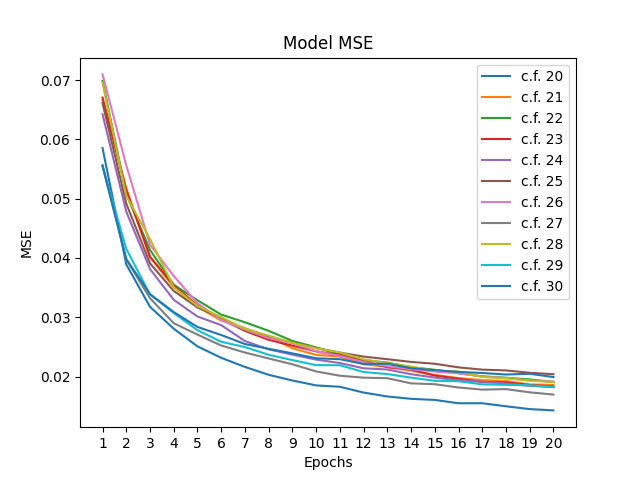
\includegraphics[width=3.5in]{multiacc.png}
\captionsetup{justification=centering}                                                                                         
\caption{MSE vs. number of epochs vs. compression factor}
\label{fig:multiacc}
\end{figure}

\begin{figure}[ht!]
\centering                                                                        
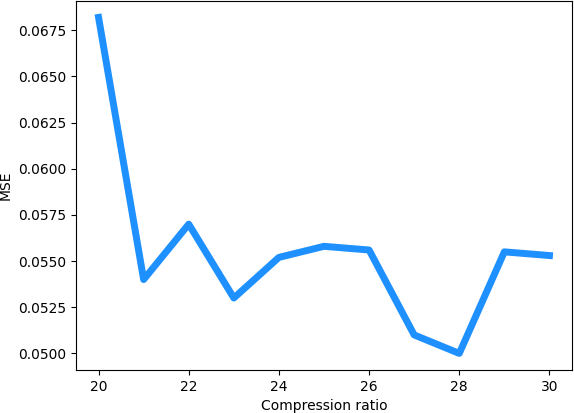
\includegraphics[width=3.5in]{mse.png}
\captionsetup{justification=centering}                                                                                                                              
\caption{MSE with different compression factors}
\label{fig:mse}                                                                                                                                         
\end{figure}


Figure \ref{fig:auto} shows the final architecuture of the autoencoder: 1092 neurons for input, 256 and 128 for encoding, 54 for storing the compressed knowledge, 128, 256 and 512 for decompression and 1092 for output.\par
All the layers used \texttt{LeakyReLU} with $\alpha=0.01$ as activation function. The output layer used a \emph{Sigmoid} that better represents values between 0 and 1.

\subsection{Training}
For the training phase we used \emph{Adam} but with \emph{binary crossentropy} loss function. \emph{Binary crossentropy}, based on the logarithmic operation, 
better avoids the effects present in the \emph{Sigmoid} function, that is based on the exponential function.

\begin{figure}[ht!]
\centering                                                                        
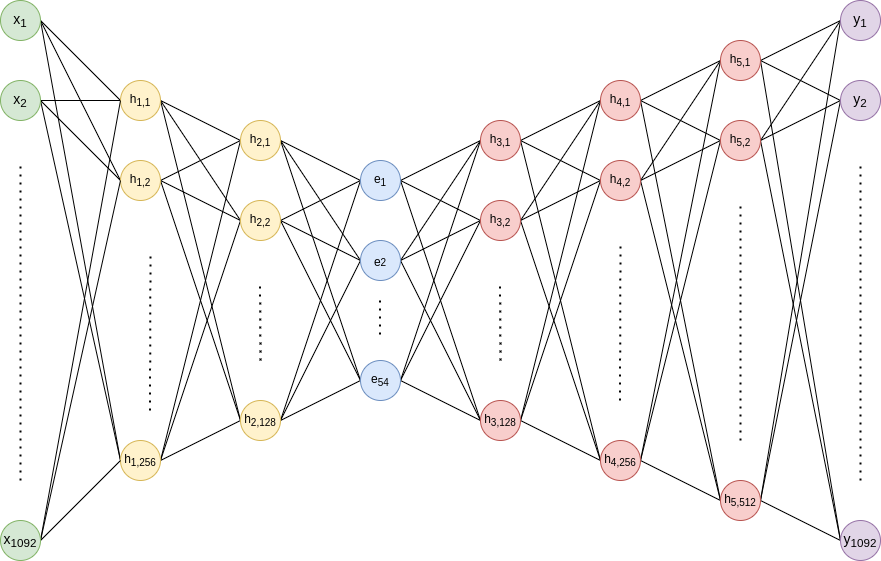
\includegraphics[width=3.5in]{auto.png}
\captionsetup{justification=centering}
\caption{Final architecture of the autoencoder: in green the input, in yellow the encoders, in blue the latent layer, in red the encoder and in purple the output}
\label{fig:auto}
\end{figure}

\subsection{Evaluation}
The best way to evaluate the autoencoder, along with plotting the loss and the MSE, is to visualize the results (Figure \ref{fig:reproduce}). In the first row
there are 10 samples from the test set while in the second row the output of the autoencoder. The similarity between the two sequences in quite high, but we
can notice that the second row present a certain level of blurriness.


\begin{figure}[ht!]
\centering                                                                        
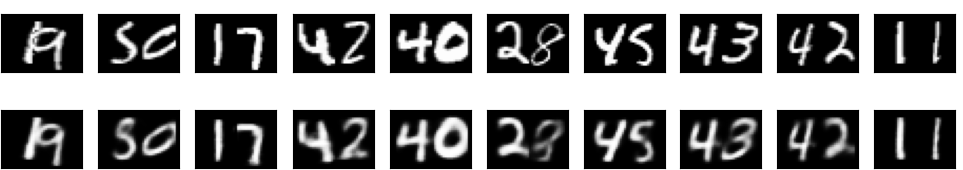
\includegraphics[width=3.5in]{reproduce.png}
\captionsetup{justification=centering}
\caption{First row: original test data. Second row: the same input but reproduced by the autoencoder.}
\label{fig:reproduce}
\end{figure}

\subsection{Generation}
In order to generate random new samples, we trained the autoencoder as previously and used only the second part of the architecture, that is 
from the encoded layer to the output (Figure \ref{fig:generator})


\begin{figure}[ht!]
\centering                                                                        
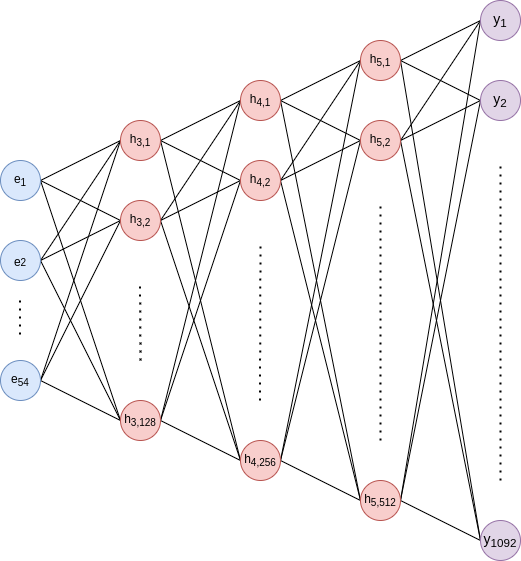
\includegraphics[width=2.5in]{generator.png}
\captionsetup{justification=centering}
\caption{}
\label{fig:generator}
\end{figure}

We fed the model with random numbers with two different distributions: the first is a uniform distribution from 0 to 1 and the second a custom one we describe later.\par
The random input with uniform distribution gave the results shown in Figure \ref{fig:unif}

\begin{figure}[ht!]
\centering                                                                        
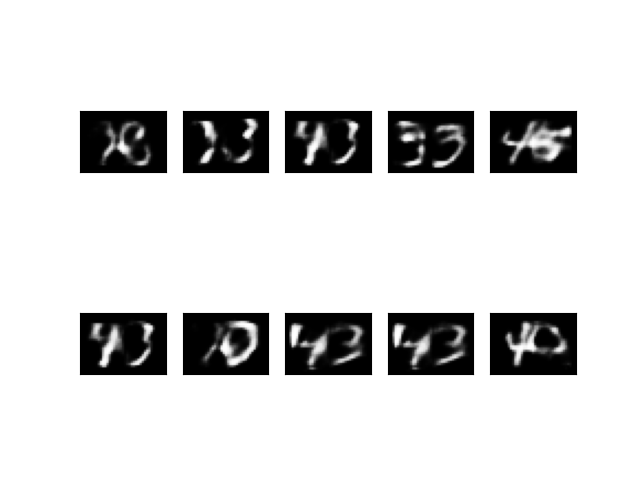
\includegraphics[width=3.5in]{unif.png}
\captionsetup{justification=centering}
\caption{New samples generated from a uniform distribution}
\label{fig:unif}
\end{figure}

We can distinguish some numbers (like 38, 33, 40, 43 and 45) but they are blurry, lowly defined and redundant.

\begin{figure}[ht!]
\centering                                                                        
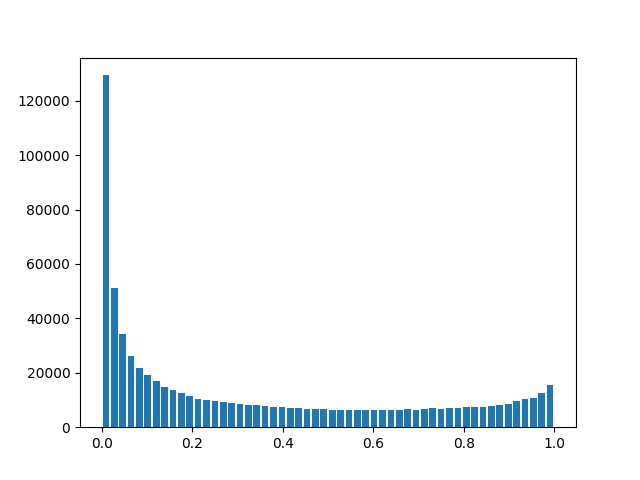
\includegraphics[width=3.5in]{enco.png}
\captionsetup{justification=centering}
\caption{}
\label{fig:enco}
\end{figure}

Because results were not exhaustive, we andalyzed the distribution in the encoded layer after having fed the network with the entire
test set. Figure \ref{fig:enco} demonstrate that the distribution is far from being uniform.


So we implemented a custom distribution that tried to emulate the real distribution
present in the encoded layer after feeding the model with entire test set. Algorithm \ref{alg:ran} describes the procedure.

\begin{algorithm}[h]
\SetAlgoLined
\KwData{$P \textnormal{ matrix of predictions over } X_{test}$, $n \in \mathbb{N} \textnormal{ number of encodings}$}
\KwResult{\emph{$E \textnormal{ matrix of random } $n$ \textnormal{ encodings}$}}

$E \gets \mathcal{M}(n \times 54)$\;
\For{$i \gets 0$ \textbf{to} $n$}{

\For{$j \gets 0$ \textbf{to} $54$}{

$column \gets P_{*,j}$\;
$m \gets \mu(column)$\;
$s \gets \sigma(column)$\;
$E_{i,j} \gets random(\mathcal{N}(m, s))$
}

}



\Return $E$\;

\caption{Simulator}\label{alg:ran}
\end{algorithm}

The procedure calculates a new matrix of encodings, generated by a normal distribution $\mathcal{N}(\mu, \sigma)$ on each column, where $\mu$ and $\sigma$ are calculated on the same column of the matrix of encodings. Since the first dimension describes different sequence, what is important is to maintain the distribution
of each column. That's because the weights in the encoding layer (and in any other) cannot be permutated without affecting the final result of the model. That's why we emulated the distribution by column, assuming that is normally distributed (which is probably not, but this should require more time in investigation). 


\begin{figure}[ht!]
\centering                                                                        
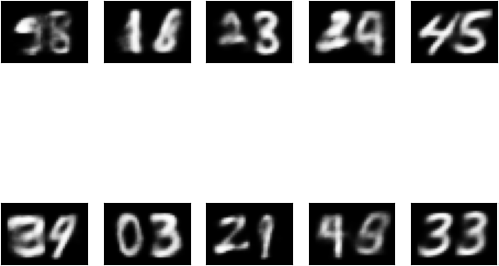
\includegraphics[width=3.5in]{gen.png}
\captionsetup{justification=centering}
\caption{}
\label{fig:gen}
\end{figure}

Figure \ref{fig:gen} shows the results, which are way better than the ones generated with a uniform distribution. We can find sharper shapes, a little bit of more
diversity in the digits (although there are many $3$s). What is very interesting is the appearance of a $98$, even if the network has been trained on numbers between $1$ and $50$. This suggests that the order of the weights matters but it doesn't describe the order of the digits; that is quite predictable since the layers are densely-connected and every neuron can affect any other neuron of the next layer.

\end{document}









